\documentclass{standalone}
\usepackage{tikz}
\usetikzlibrary{calc, shapes, patterns}

\begin{document}
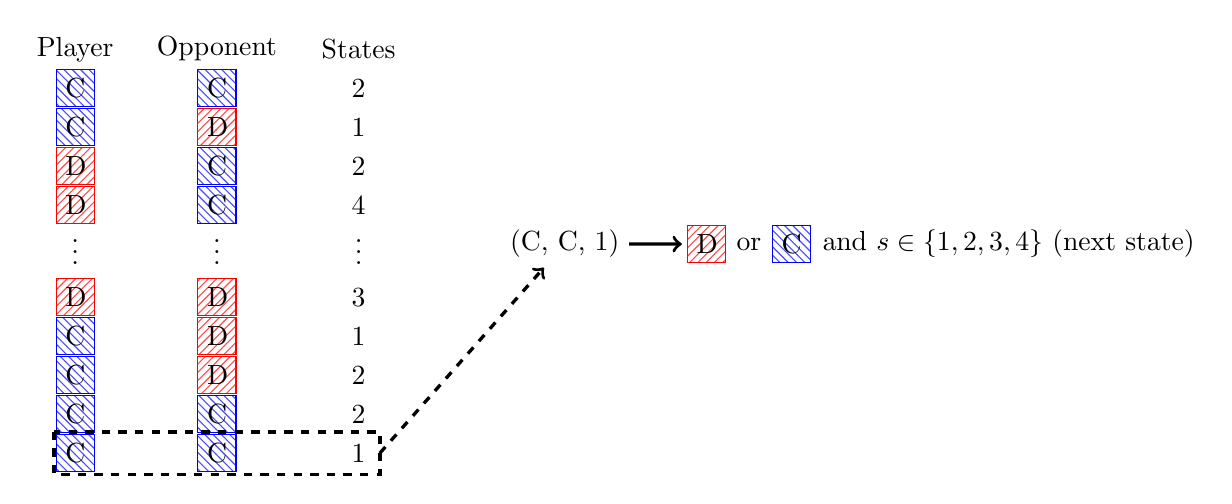
\begin{tikzpicture}[scale=.9]
    \tikzstyle{cooperator} = [rectangle, pattern=north west lines, pattern
        color=blue!70, draw=blue, text width=.25cm, outer sep = 2pt]
    \tikzstyle{defector} = [rectangle, pattern=north east lines, pattern
        color=red!70, draw=red, text width=.25cm, outer sep = 2pt]


    % Histories ----------------------------------------
    \node (A) at (-.5, 0) {Player};
    \node (A1) at ($(A) + (0, -.55)$) [cooperator] {C};
    \node (A2) at ($(A1) + (0, -.55)$) [cooperator] {C};
    \node (A3) at ($(A2) + (0, -.55)$) [defector] {D};
    \node (A4) at ($(A3) + (0, -.55)$) [defector] {D};
    \node (A5) at ($(A4) + (0, -.55)$) {$\vdots$};
    \node (A6) at ($(A5) + (0, -.75)$) [defector] {D};
    \node (A7) at ($(A6) + (0, -.55)$) [cooperator] {C};
    \node (A8) at ($(A7) + (0, -.55)$) [cooperator] {C};
    \node (A9) at ($(A8) + (0, -.55)$) [cooperator] {C};
    \node (A10) at ($(A9) + (0, -.55)$) [cooperator] {C};


    \node (B) at ($(A) + (2, 0)$) {Opponent};
    \node (B1) at ($(B) + (0, -.55)$) [cooperator] {C};
    \node (B2) at ($(B1) + (0, -.55)$) [defector] {D};
    \node (B3) at ($(B2) + (0, -.55)$) [cooperator] {C};
    \node (B4) at ($(B3) + (0, -.55)$) [cooperator] {C};
    \node (B5) at ($(B4) + (0, -.55)$) {$\vdots$};
    \node (B6) at ($(B5) + (0, -.75)$) [defector] {D};
    \node (B7) at ($(B6) + (0, -.55)$) [defector] {D};
    \node (B8) at ($(B7) + (0, -.55)$) [defector] {D};
    \node (B9) at ($(B8) + (0, -.55)$) [cooperator] {C};
    \node (B10) at ($(B9) + (0, -.55)$) [cooperator] {C};
    % ---------------------------------------------------

    % States
    \node (S) at ($(B) + (2, 0)$) {States};
    \node (S1) at ($(S) + (0, -.55)$)  {2};
    \node (S2) at ($(S1) + (0, -.55)$)  {1};
    \node (S3) at ($(S2) + (0, -.55)$)  {2};
    \node (S4) at ($(S3) + (0, -.55)$)  {4};
    \node (S5) at ($(S4) + (0, -.55)$) {$\vdots$};
    \node (S6) at ($(S5) + (0, -.75)$)  {3};
    \node (S7) at ($(S6) + (0, -.55)$)  {1};
    \node (S8) at ($(S7) + (0, -.55)$)  {2};
    \node (S9) at ($(S8) + (0, -.55)$)  {2};
    \node (S10) at ($(S9) + (0, -.55)$)  {1};
    % ---------------------------------------------------


    % Identifying inputs --------------------------------
    \draw[very thick, black, dashed] ($(A10) + (-.3, .3)$)  rectangle ($(S10) + (.3, -.3)$);

    %% Strategy inputs
    \node (inputs) at ($(S5) + (2, 0)$) [right] {(C, C, 1)};

    \draw [very thick, black, dashed, ->] ($(S10) + (.3, 0)$) -- (inputs);

    % output
    \node (output) at ($(inputs) + (2, 0)$) [defector] {D};
    \node (or) at ($(output) + (.6, 0)$) {or};
    \node (c) at ($(or) + (.6, 0)$) [cooperator] {C};
    \node at ($(c) + (0.3, 0)$) [right] {and \(s\in\{1, 2, 3, 4\}\) (next state)};

    %\node (action_output) at ($(inputs) + (1.5, 0)$) [cooperator] {C};
    %\node (state_output) at ($(action_output) + (.55, 0)$) {4};

    \draw [->, very thick] (inputs) -- (output);
\end{tikzpicture}
\end{document}
